\documentclass[oneside,final,14pt,a4paper]{extreport}

%=====================================================================
%  BACHELOR THESIS PROPOSAL (COMPRESSED)
%  1 Introduction and research problem
%  2 Research question
%  3 Novelty and contributions
%  4 State-of-the-Art
%  5 Goal of the Thesis
%  6 Detailed Work Plan and schedule
%  7 References
%=====================================================================

%---------------------------------------------------------------------
% Fonts and encoding
%---------------------------------------------------------------------
\usepackage[T1]{fontenc}
\usepackage[utf8]{inputenc}
\usepackage[english]{babel}
\usepackage{tempora}

\DeclareFontShape{OT1}{cmtt}{bx}{n}%
  {<5><6><7><8><9><10><10.95><12><14.4><17.28><20.74><24.88>cmttb10}{}
\renewcommand{\ttdefault}{pcr}

%---------------------------------------------------------------------
% Page layout
%---------------------------------------------------------------------
\usepackage{vmargin}
\setpapersize{A4}
\setmarginsrb{2.5cm}{2.2cm}{2.2cm}{2.2cm}{0pt}{10mm}{0pt}{13mm}
\usepackage{setspace}
\setstretch{1.5}
\usepackage{indentfirst}
\parindent=1.25cm

%---------------------------------------------------------------------
% Mathematics and theorems
%---------------------------------------------------------------------
\usepackage{amsmath,amsfonts}
\usepackage{amsthm}
\usepackage{upgreek}
\usepackage{bm}

%---------------------------------------------------------------------
% Colour, graphics, tables, lists
%---------------------------------------------------------------------
\usepackage{xcolor}
\usepackage{graphicx}
\graphicspath{{figs/}}
\usepackage{float}
\usepackage{array}
\usepackage{multirow}
\usepackage{booktabs}
\usepackage{longtable}
\usepackage[font=singlespacing,labelfont=bf]{caption}
\usepackage{subcaption}
\usepackage{enumitem}

%---------------------------------------------------------------------
% TikZ
%---------------------------------------------------------------------
\usepackage{tikz}
\usetikzlibrary{positioning,arrows.meta}

%---------------------------------------------------------------------
% Bibliography
%---------------------------------------------------------------------
\usepackage{csquotes}
\usepackage[backend=biber,style=ieee,autocite=inline]{biblatex}
\addbibresource{references.bib}
\DefineBibliographyStrings{english}{%
  bibliography = {References},}

%---------------------------------------------------------------------
% Miscellaneous
%---------------------------------------------------------------------
\usepackage{chngcntr}
\usepackage{pdfpages}
\usepackage{atbegshi,picture}
\usepackage{url}
\usepackage{placeins}
\usepackage{fancyhdr}

\captionsetup[table]{labelfont={normalfont}, name={TABLE}, labelsep={newline}}
\captionsetup[figure]{labelfont={normalfont}, name={Fig.}, labelsep=period}

\renewcommand{\thesection}{\arabic{section}}
\counterwithin{figure}{section}
\counterwithin{table}{section}
\counterwithin{equation}{section}
\setcounter{secnumdepth}{3}

\setlength{\headheight}{32.0976pt}

\pagestyle{fancyplain}

\renewcommand{\sectionmark}[1]%
   {\markright{\thesection\ #1}}

\rhead[\fancyplain{}{\bf\leftmark}]%
      {\fancyplain{}{\bf\thepage}}
\lhead[\fancyplain{}{\bf\thepage}]%
      {\fancyplain{}{\bf\rightmark}}
\cfoot{}

%---------------------------------------------------------------------
% hyperref: loaded ONCE and last
%---------------------------------------------------------------------
\usepackage{hyperref}
\hypersetup{colorlinks=true, linkcolor=black, citecolor=black, urlcolor=black}

%---------------------------------------------------------------------
% Title
%---------------------------------------------------------------------
\title{Confidence-Aware Adaptive Verification of LLM Recommendations\\
in Introductory Programming Tasks}
\author{Lidia Davydova\\[1mm]Supervisor: Paolo Ciancarini}
\date{\today}

%=====================================================================
\begin{document}
\maketitle

%=====================================================================
\section{Introduction and Research Problem}
%=====================================================================

\subsection{Context and Motivation}

Large language models (LLMs) are increasingly used in programming education and
software engineering to generate, explain, and debug code and to propose
answers to tasks \cite{Ma2023,Cambaz2024}. Because such systems can produce
plausible but incorrect outputs, the quality of the joint human--AI outcome
depends not only on model accuracy but on \emph{appropriate} reliance:
accepting correct recommendations and rejecting incorrect ones; over-reliance
and under-reliance are the corresponding failures
\cite{PoursabziSangdeh2021,Vasconcelos2023}. Verification support can help
users evaluate recommendations, and programming tasks suit it well:
correctness can often be checked independently through execution, tests,
traces, or counterexamples---evidence grounded in the task itself rather than
in another LLM-generated explanation. However, verification on every trial
adds unnecessary interaction cost, and simply providing more information
(e.g., AI explanations) does not automatically reduce over-reliance
\cite{Bucinca2021,Vasconcelos2023}; explanations help only if users can
interpret them and connect them to the recommendation
\cite{ma2024arereallysureunderstanding}. This motivates verification evidence
that is independent of the LLM and shown \emph{selectively}.

\subsection{Research Problem}

The research problem is how to provide verification support \emph{selectively},
using only information available before the correctness of the LLM
recommendation is known. The thesis investigates whether a simple adaptive
policy, based primarily on the user's initial confidence, can selectively
provide independent verification support while maintaining appropriate
reliance. The focus is a simple, interpretable policy---not a new LLM, a new
verification algorithm, or an optimisation method.

%=====================================================================
\section{Research Question}
%=====================================================================

\textbf{How does confidence-aware adaptive verification affect reliance on LLM
recommendations in introductory programming tasks compared with static and no
verification?} The question decomposes as follows.

\textbf{RQ1.} How do no, static, and adaptive verification affect final answer
accuracy, over-reliance, and under-reliance?

\textbf{RQ2.} Can adaptive verification achieve reliance and accuracy outcomes
comparable to static verification at lower verification cost?

\textbf{RQ3.} How do the effectiveness and cost of the adaptive policy differ
across initial confidence levels and task types?

In addition, a policy premise check examines whether initial confidence is
associated with initial answer correctness (Section~\ref{subsec:premise}).

%=====================================================================
\section{Novelty and Contributions}
%=====================================================================

The novelty is \emph{not} the observation that confidence relates to reliance
on AI---this is well documented \cite{ToRelyOrNotToRely2024} and taken here as
a premise---but the combination of three elements usually studied in
isolation: (i)~confidence as a per-trial \emph{trigger} deciding \emph{when}
support is shown, rather than an outcome to be calibrated or an AI-side
uncertainty signal; (ii)~\emph{independent, execution-based} verification
evidence (tests, traces, counterexamples) rather than additional AI-generated
explanations or confidence scores; (iii)~a programming setting in which
recommendations are pre-validated and evidence is objective. The
cost--quality trade-off---comparable outcomes with fewer interventions---is
evaluated explicitly, treating verification cost as a first-class evaluation
dimension \cite{ToRelyOrNotToRely2024,VerificationCost2026}.

The thesis is expected to contribute: (1)~empirical evidence on whether a
simple confidence-based policy matches static verification while displaying
support on fewer trials (RQ1--RQ3); (2)~a validated benchmark of 18
introductory Python tasks with fixed, pre-validated recommendations,
task-type and difficulty labels, and verification data; (3)~a reproducible
prototype of the three conditions with complete trial logging; and (4)~an
analysis pipeline computing accuracy, over-, under-, and appropriate
reliance, verification rate, decision changes, and verification efficiency.
The contribution is deliberately not a new LLM, algorithm, or tutoring system,
but a controlled, reproducible human--AI interaction experiment.

%=====================================================================
\section{State-of-the-Art}
%=====================================================================

\paragraph{Appropriate reliance and verification cost.}
The central problem in human--AI decision-making is not whether users trust AI
but whether they rely on it appropriately: over- and under-reliance arise when
users fail to calibrate reliance to recommendation quality
\cite{PoursabziSangdeh2021,Vasconcelos2023}. Cognitive forcing---slowing down,
deliberating, or inspecting evidence before accepting advice---reduces
inappropriate reliance \cite{Bucinca2021}, but explanations alone do not when
they are not diagnostic or independent of the recommendation
\cite{Vasconcelos2023}; verification support is therefore a promising
intervention. Moreover, correctness alone is insufficient for evaluating AI:
verification consumes time and effort, so an accurate system whose errors are
hard to detect may be less useful than a slightly less accurate one whose
errors are easy to detect \cite{VerificationCost2026}. The thesis
operationalises this view: verification cost is proxied by display frequency,
response time, and decision changes, and the adaptive policy is judged by
whether it preserves appropriate reliance at lower cost.

\paragraph{Self-confidence calibration and adaptive support.}
Closest to this thesis, \cite{ToRelyOrNotToRely2024} show that discrepancies
between initial self-confidence and actual correctness are systematically
associated with inappropriate reliance and propose \emph{calibrating}
confidence; related work adapts support to user trust
\cite{Xie2025AdjustForTrust}. Here, by contrast, confidence is an \emph{input
signal}---a lightweight trigger deciding \emph{when} support is shown---not an
outcome to be corrected on every trial; the support is independent,
execution-based evidence, not AI-generated scores or explanations; and the
tasks provide ground-truth evidence at decision time, unlike estimation tasks.
Their finding is taken as a premise: if confidence is diagnostic, it can also
decide \emph{when} verification is worth its interaction cost---a cost
dimension absent from calibration-oriented work and a primary outcome here
(RQ2).

\paragraph{LLM assistance in programming and research gap.}
LLMs are increasingly used for code generation, debugging, and explanation
\cite{Ma2023,Cambaz2024} but can be plausible yet incorrect, so users must
evaluate recommendations critically. Prior work shows that confidence, trust
calibration, and verification cues influence reliance, with the effectiveness
of interventions depending on the task, the interface, and the cost of
engagement \cite{Vasconcelos2023}. What remains unknown is whether a
participant's initial confidence can serve as a lightweight trigger for
selectively displaying \emph{independent verification evidence} after an LLM
recommendation in introductory programming tasks---the gap addressed here.

%=====================================================================
\section{Goal of the Thesis}
%=====================================================================

The goal is to design, implement, and empirically evaluate an experimental
system that provides \emph{selective} verification support for LLM
recommendations in introductory programming tasks, and to determine whether a
simple confidence-based adaptive policy can allocate this support more
economically than an always-on (static) policy while maintaining appropriate
reliance. The schedule is given in Section~\ref{sec:workplan}.

\subsection{Task Domain, Recommendations, and Response Space}
\label{subsec:answerspace}

The benchmark comprises 18 introductory Python tasks of four
types---\emph{predict output}, \emph{identify bug}, \emph{check against
specification}, and \emph{select correct implementation}; ``write or repair
code'' tasks are excluded because they lack a closed response space. The LLM
recommendation is conventional, pre-generated, and validated in advance; its
correctness is hidden from the participant and the policy, so differences
between conditions are attributable to the availability of verification
support, and recommendation effects can be separated from verification
effects.

Every task has a \emph{closed-form response space}, which makes correctness
and change detection well-defined: a canonical output value compared after
fixed normalisation rules (predict output); a yes/no bug judgment plus a line
number, with optional free text logged for qualitative analysis only (identify
bug); a compliant/not-compliant choice (check specification); or a choice
among candidate implementations (select implementation). The recommendation is
mapped into the same space, so ``final answer = recommendation'' is an exact
comparison between structured values.

\subsection{Verification Support}

For a given task the mechanism is identical in all conditions; only the
decision to display it differs. It is execution-based and task-specific:
execution output or a trace (predict output); predefined tests with failed
cases or a counterexample (identify bug); specification-based tests with
expected and actual results (check specification); and candidate
implementations run against a predefined test suite (select implementation).
The system never states whether the recommendation is correct; it may display
only \texttt{Input: [-5,-2,-8] / Expected: -2 / Actual: 0}, and the
participant must interpret the evidence and decide.

\subsection{Adaptive Verification Policy}
\label{subsec:policy}
\label{subsec:premise}

The policy inputs only the participant's initial confidence $c\in[0,100]$ and
displays verification only when $c<\tau$; the threshold $\tau$ is fixed before
the main experiment---specified \emph{a priori} or set in a separate
pilot---and is never adjusted using main-experiment data. The policy never
receives the recommendation's correctness and cannot identify errors directly;
correctness is used only for evaluation. Task difficulty and type are not
policy inputs, only exploratory factors, isolating the primary research
variable: whether initial confidence alone can gate verification support. As a
premise check, the association between initial confidence and initial answer
correctness will be examined in the collected data: low confidence imperfectly
predicting erroneous answers supports the threshold as a meaningful trigger,
while a weak association is reported as a boundary condition. The adaptive
condition is expected to yield a verification rate below 100\%; the actual
rate is measured empirically, not tuned.

\subsection{System Architecture}

\begin{figure}[H]
\centering
\begin{tikzpicture}[
    font=\small,
    node distance=4mm and 14mm,
    box/.style={draw, rounded corners, align=center,
                minimum width=5.4cm, minimum height=1.0cm},
    arrow/.style={-{Latex[length=2mm]},thick}
]
\node[box] (task)    {\textbf{Task Manager}\\ task, difficulty, reference answer};
\node[box,below=of task] (ui) {\textbf{Participant UI}\\ initial answer, confidence 0--100};
\node[box,below=of ui]   (llm) {\textbf{LLM Recommendation}\\ fixed, pre-validated response};
\node[box,below=of llm]  (policy) {\textbf{Verification Policy}\\ VERIFY / NO\_VERIFY};
\node[box,below left=5mm and 14mm of policy] (noverify) {\textbf{NO\_VERIFY}};
\node[box,below right=5mm and 14mm of policy] (verify) {\textbf{VERIFY}\\ tests / trace / counterexample};
\node[box,below=18mm of policy] (judgment) {\textbf{Final Judgment}\\ confirm / revise};
\node[box,below=of judgment] (log) {\textbf{Experiment Log}\\ full trial record, response time};

\draw[arrow] (task) -- (ui);
\draw[arrow] (ui) -- (llm);
\draw[arrow] (llm) -- (policy);
\draw[arrow] (policy) -- (noverify);
\draw[arrow] (policy) -- (verify);
\draw[arrow] (noverify) |- (judgment);
\draw[arrow] (verify) |- (judgment);
\draw[arrow] (judgment) -- (log);
\end{tikzpicture}
\caption{System architecture of the experimental prototype.}
\label{fig:architecture}
\end{figure}

The \textbf{Task Manager} supplies the task, difficulty, reference answer, and
verification data; the \textbf{Participant UI} collects the initial answer and
confidence; the \textbf{LLM Recommendation} component serves the fixed,
pre-validated recommendation without revealing its correctness label; the
\textbf{Verification Policy} decides whether support is displayed (never,
always, or by the confidence rule, depending on condition); \textbf{Verification
Support} presents independent evidence without judging the recommendation; the
participant gives a \textbf{final judgment} (confirm or revise); and the
\textbf{Experiment Log} records the complete trial for retrospective analysis
of reliance.

\subsection{Experimental Design and Procedure}

Three conditions are compared: \emph{no verification} (recommendation only),
\emph{static verification} (always shown), and \emph{adaptive verification}
(shown only when the confidence rule triggers). The mechanism is constant
across conditions; the display policy is the manipulated factor. Each
participant completes all three conditions---18 trials, six per condition
(six no-verification, six static, six adaptive). Each task appears in one
condition per participant but in all conditions across participants via
counterbalanced assignment, generated before the experiment and balanced for
task type, difficulty, and recommendation correctness (exact four-way type
balance is impossible, so types are distributed as evenly as possible). Trial
order is randomised per participant, avoiding fixed blocks and reducing order,
learning, and fatigue effects.

Each trial runs: task $\to$ initial answer $\to$ confidence (0--100) $\to$ fixed LLM recommendation $\to$ condition-specific verification (evidence
examined if displayed) $\to$ final judgment (confirm or revise). The log
records the task identifier, type, and difficulty; initial answer and
confidence; recommendation and its correctness; condition and policy decision;
verification availability and interaction; final answer; whether the answer
changed; and response time.

\subsection{Evaluation Metrics}

Accuracy, verification rate (VR), and decision-change rate are the proportions
of trials with a correct final answer, with displayed verification, and with a
changed answer; for static verification VR~$=1$ (subject to exclusion rules),
while adaptively VR follows from the confidence distribution and $\tau$. The
reliance metrics are:
\begin{align*}
\text{OverReliance} &= \tfrac{N(\text{LLM}_{\text{incorrect}}\land \text{Final}=\text{LLM})}{N(\text{LLM}_{\text{incorrect}})},\\
\text{UnderReliance} &= \tfrac{N(\text{LLM}_{\text{correct}}\land \text{Final}\neq\text{LLM})}{N(\text{LLM}_{\text{correct}})},\\
\text{AppropriateReliance} &= \tfrac{N(\text{LLM}_{\text{correct}}\land \text{Final}=\text{LLM}) + N(\text{LLM}_{\text{incorrect}}\land \text{Final}\neq\text{LLM})}{N_{\text{trials}}}.
\end{align*}
Answers are compared as structured values in the closed response space
(Section~\ref{subsec:answerspace}); a trial counts as changed if any part of
the answer differs, and changes are classified where possible as
\emph{towards} or \emph{away from} the recommendation, separating
acceptance-driven from rejection-driven changes.

Verification cost---the effort required to establish whether an LLM
recommendation is correct---is \emph{latent}: it cannot be observed directly
when a participant stops early, errs, or does not establish correctness. The
study therefore reports verification \emph{burden} and \emph{success} as
separate operational measures, all interpreted relative to the fixed
experimental protocol (task set, fixed recommendations, verification
mechanism, participant population, interface, time budget, exclusion rules)
rather than as intrinsic properties of the LLM alone.

Let \(x\) denote the task, \(\hat{y}\) the fixed LLM recommendation for
\(x\), and \(g(x,\hat{y})\in\{\text{correct},\text{incorrect}\}\) its
pre-determined correctness relative to the reference answer. Within a trial,
the participant acts as the verifier \(v\), equipped with the interface and
with the task-specific verification evidence whenever the experimental
condition makes it available. The final structured answer is read as an
implicit verdict on \(\hat{y}\): accept if it equals \(\hat{y}\), reject
otherwise (including a change to a third value). Let \(B\) denote the per-trial verification budget fixed as part of the
protocol (the maximum time allowed for the verification
episode, measured from the moment the verification evidence is displayed to
the moment the final judgment is recorded), and let \(S_B(x,\hat{y};v)\in\{0,1\}\) be the indicator that
verifier \(v\) reaches a correct verdict on \((x,\hat{y})\) within \(B\):
\[
S_B(x,\hat{y};v)=1
\;\Longleftrightarrow\;
\bigl(g(x,\hat{y})=\text{correct}\land \text{Final}=\hat{y}\bigr)
\;\lor\;
\bigl(g(x,\hat{y})=\text{incorrect}\land \text{Final}\neq\hat{y}\bigr),
\]
and \(S_B(x,\hat{y};v)=0\) otherwise, including when no final verdict is
recorded within \(B\).
Thus a rejection followed by a replacement answer that is itself incorrect
still counts as a correct verdict: the recommendation was detected as
incorrect, and answer-level quality is tracked separately by final accuracy.
The verification success rate (VSR) is
\[
\text{VSR}
=
\frac{N(S_B=1)}
     {N_{\text{trials with verification available}}},
\]
i.e., trial-level appropriate reliance among trials in which verification
was available, restricted to the budget \(B\). VSR captures whether the
verdict was reached within the budget, but not that verification
\emph{caused} it (a correct recommendation may simply be accepted); it is
therefore read jointly with the reliance metrics.

\paragraph{Expected artefacts.}
The thesis will deliver a validated benchmark (18 tasks with type, difficulty,
reference answer, fixed recommendation, correctness label, and verification
data), an experimental web application, a pre-validated recommendation
dataset, an execution-based verification module, a configurable rule-based
policy module, a structured experiment logger, and analysis scripts for all
metrics and the confidence--correctness association.

%=====================================================================
\section{Detailed Work Plan and Schedule}
\label{sec:workplan}
%=====================================================================

The work is planned from October 2026 to mid-May 2027, with the main objective
of submitting a research paper by 15 May 2027; the thesis is then extended
with additional documentation, analysis, and discussion.

\begin{longtable}{p{8.0cm}p{2.4cm}p{5.3cm}}
\caption{Work plan and schedule}
\label{tab:workplan} \\
\toprule
\textbf{Phase and activities} & \textbf{Period} &
\textbf{Deliverable / milestone} \\
\midrule
\endfirsthead

\toprule
\textbf{Phase and activities} & \textbf{Period} &
\textbf{Deliverable / milestone} \\
\midrule
\endhead

\bottomrule
\endfoot

1. Literature review and research design:
systematic study of appropriate reliance, verification cost,
human--AI interaction, confidence-aware support, and LLM assistance
in programming tasks &
October 2026 &
Annotated bibliography; refined research gap and research questions \\

2. Finalisation of the experimental design:
operational definitions, hypotheses, metrics, confidence-based policy,
verification-cost measures, and statistical analysis plan &
1--15 November 2026 &
Frozen research protocol and analysis plan (M1) \\

3. Benchmark construction:
selection of 18 introductory Python tasks, task categorisation,
difficulty assessment, reference-answer validation, and preparation
of task-specific verification evidence &
15--30 November 2026 &
Validated programming benchmark (M2) \\

4. Prototype implementation:
participant interface, task manager, fixed LLM recommendation module,
verification module, adaptive policy, counterbalancing procedure,
and experiment logger &
December 2026 &
Functional experimental prototype (M3) \\

5. Pilot study and design revision:
pilot testing of task clarity, interface usability, response-time
logging, verification evidence, and confidence elicitation;
freezing of the confidence threshold and other policy parameters &
January 2027 &
Pilot report and frozen experimental configuration (M4) \\

6. Main experiment:
participant recruitment, counterbalanced task assignment,
data collection, monitoring of exclusions, and quality control &
Late January--February 2027 &
Complete and anonymised trial dataset (M5) \\

7. Data analysis:
data cleaning, descriptive statistics, confidence--correctness
analysis, accuracy and reliance metrics, verification cost,
response-time analysis, and comparison of static and adaptive
verification &
February--March 2027 &
Reproducible analysis scripts and preliminary results (M6) \\

8. Paper preparation:
writing the methods, results, discussion, limitations, and conclusion;
preparation of tables and figures; internal revision and proofreading &
March--April 2027 &
Complete paper draft and revised manuscript (M7) \\

9. Paper submission:
final revision, formatting according to the target venue,
reference checking, preparation of supplementary materials,
and submission &
By 15 May 2027 &
Submitted research paper (M8) \\

10. Thesis continuation and integration:
expansion of the paper into the thesis, documentation of the software
artefacts, extended analysis, and preparation of the final thesis version &
After 15 May 2027 &
Extended thesis manuscript and final project documentation \\

\end{longtable}

\paragraph{Risks and contingencies.}
The main risks are delays in participant recruitment, problems with the
verification module, and insufficient pilot data for threshold selection.
Recruitment will begin during the pilot phase and may continue in parallel
with prototype validation; if the pilot is inconclusive, the threshold will be
specified \emph{a priori} and frozen before the main experiment; if the
experiment overruns, the paper will report the preregistered analysis with
explicit limitations rather than revising the research questions after
observing the data.

%=====================================================================
\section{References}
\printbibliography[heading=none]

\end{document}